\chapter{Prezentarea contribuțiilor autorului}
\label{cap:contributii}
În acest capitol se face prezentarea contribuțiilor autorului: un studiu comparativ a metodelor existente de detecția obiectelor și segmentarea semantică a imaginilor bazate pe rețele neuronale convoluționale. Se vor analiza algoritmii de inteligență artificială deorece performanța acestora în domeniul prelucrării imaginilor depășește semnificativ orice altă metodă (algoritmi de nivel mai jos, cum ar fi algoritmii de thresholding).

\section{Precizări asupra conținutului și a modului de organizare}

Titlul acestui capitol nu este unul impus și nici nu corespunde neapărat unui singur capitol. Titlul indică mai degrabă o parte (importantă și centrală, de altfel) a lucrării, în care se prezintă ceea ce s-a realizat efectiv: contribuțiile autorului. Organizarea acestei părți este dependentă și specifică fiecărei lucrări în parte și este stabilită de către fiecare autor după cum i se pare mai potrivit pentru tema lui. Ea poate cuprinde prezentarea unor concepte teoretice (unelte sau tehnici matematice folosite în lucrare, prezentarea sau introducerea unor concepte teoretice etc.), o analiză a diferitelor metode/algoritmi/tehnologii etc. luate în considerare sau dezvoltate de către autor, o prezentare a unui design (mai mult sau mai puțin detaliat) sau chiar detalii a unei eventuale implementări/prototip, dacă e cazul.

Trebuie remarcat însă faptul că această parte reprezintă contribuția personală a autorului, chiar dacă ea constă de exemplu doar dintr-o analiză comparativă a unor metode/algoritmi, și în nici un caz ea nu poate fi sinteza unor texte preluate din alte surse. Prin urmare, orice informații sunt prezentate aici, ele trebuie să corespundă cel puțin unei interpretări/analize critice personale a autorului, dacă nu chiar unor idei originale ale acestuia. 

\subsection{Dimensiune}

Împreună cu capitolul (partea) următor reprezintă cca. 70\% din lucrare. 


\section{Examples: lists, figures, tables, equations}

Așa arată o listă de elemente nenumerotate:
\begin{itemize}
  \item element 1
  \item element 2
  \item \dots
\end{itemize}


Așa arată o listă de elemente numerotare:
\begin{itemize}
  \item element 1
  \item element 2
  \item \dots
\end{itemize}


Așa arată o listă în text: 
\begin{inparaenum}[(\itshape 1 \upshape)]
  \item element 1, 
  \item element 2, 
  \item \dots
\end{inparaenum}

\textbf{Atenție}: orice tabel, figura sau ecuație (formulă) trebuie referite \textit{explicit} în text explicit (de genul: în Figura X este ulustrat \dots, în Tabelul Y se poate vedea \dots), pentru că Latex le poate plasa chiar și pe altă pagină decât acolo unde vrem noi să ne referim la ele. Vedeți exemple de mai jos!

Tabelul~\ref{table:example} ilustrează un exemplu de tabel. Un editor on-line de tabele poate fi găsit la \url{http://www.tablesgenerator.com/}. 

\begin{table}[t]
\centering                          % tabel centrat 
\begin{tabular}{|c|c|c|c|}          % 4 coloane centrate 
\hline\hline                        % linie orizontala dubla
Case & Method\#1 & Method\#2 & Method\#3 \\ [0.5ex]   % inserare tabel
%heading
\hline                              % linie orizontal simpla
1 & 50 & 837 & 970 \\               % corpul tabelului 
2 & 47 & 877 & 230 \\
3 & 31 & 25 & 415 \\[1ex]           % [1ex] adds vertical space
\hline                              
\end{tabular}
\caption{Nonlinear Model Results}   % titlul tabelului
\label{table:example}                % \label{table:nonlin} introduce eticheta folosita pentru referirea tabelului in text; referirea in text se va face cu \ref{table:nonlin}
\end{table}

În Figura~\ref{fig:exemplu} 

\begin{figure}
    \centering
    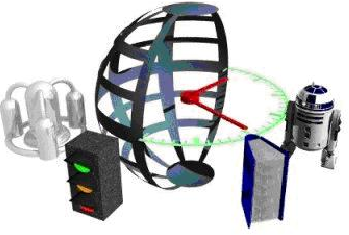
\includegraphics[width=0.5\textwidth]{image}
    \caption{Numele figurii}
    \label{fig:exemplu}
\end{figure}


Formula~(\ref{eq:example}) arată modul de calcul al lui $\Delta$:
\begin{equation} \label{eq:example}
    \Delta =\sum_{i=1}^N w_i (x_i - \bar{x})^2 .
\end{equation}


Algoritmul~\ref{alg:example} este un exemplu de descriere pseudo-cod a unui algoritm, preluat de la \href{http://en.wikibooks.org/wiki/LaTeX/Algorithms#Typesetting_using_the_algorithm2e_package}{http://en.wikibooks.org/wiki/LaTeX}. El utilizează pachetul \textit{algorithm2e}. Alternativ, puteți utiliza pachetele \textit{algorithmic} sau \textit{program}. 

\begin{algorithm}
 \KwData{this text}
 \KwResult{how to write algorithm with \LaTeX2e }
 initialization\;
 \While{not at end of this document}{
  read current\;
  \eIf{understand}{
   go to next section\;
   current section becomes this one\;
   }{
   go back to the beginning of current section\;
  }
 }
 \caption{How to write algorithms}
 \label{alg:example}
\end{algorithm}
